\chapter{Optical Flow Analysis}
Optical flow or optic flow is the pattern of apparent motion of objects, surfaces, and edges in a visual scene caused by the relative motion between an observer (an eye or a camera) and the scene\cite{lucas}.

\section{Lucas - Kanade Algorithm}
The Lucas-Kanade optical flow algorithm \cite{lucas} is a simple technique which can provide an estimate of the movement of interesting features in successive images of a scene. It associate a movement vector (u, v) to every ”interesting” pixel in the scene, obtained by comparing the two consecutive images. The Lucas-Kanade algorithm makes some implicit assumptions:

\begin{itemize}
    \item[--]The two images are separated by a small time increment ∆t, in such a way that objects have not displaced significantly (that is, the algorithm works best with slow moving objects)
    \item[--]The images depict a natural scene containing textured objects exhibiting shades of gray (different intensity levels) which change smoothly.
\end{itemize}

The algorithm does not use color information in an explicit way. It does not scan the second image looking for a match for a given pixel. It works by trying to guess in which direction an object has moved so that local changes in intensity can be explained.

Assume that we watch a scene through a square hole. The intensity \textbf{a} visible through the hole is variable.

\begin{figure}[h]
\centering
    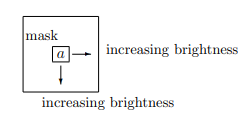
\includegraphics[scale=1]{ofa_1.png}
    \caption{Pixel intensity variation}
\end{figure}

In the next frame the intensity of the pixel has increased to \textbf{b}. It would be sensible to assume that a displacement of the underlying object to the left and up has occurred so that the new intensity b is now visible under the square hole.

\begin{figure}[h]
\centering
    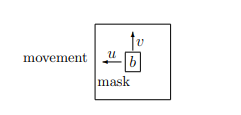
\includegraphics[scale=1]{ofa2.png}
    \caption{Movement direction}
\end{figure}

% If we know that the increase in brightness per pixel at pixel (x, y) is \(I_x(x, y)\) is the x-direction, and the increase in brightness per pixel in the y direction is \(I_y(x, y)\), we have a total increase in brightness, after a movement by u pixels in the x direction and v pixels in the y direction of:
% \begin{equation} \label{eq:eq1}
% I_x(x, y) \cdot u + I_y(x, y) \cdot v = -I_t(x, y)
% \end{equation}

% and \(I_t(x, y)\) is the local difference in intensity which is (b-a)

% a simple pixel does not usually contain enough ”structure” useful
% for matching with another pixel. It is better to use a neighborhood of pixels, for example the \(3 \times 3\) neighborhood around the pixel (x, y). In that case we set 9 linear equations:
% \begin{equation}
% I_x(x+\Delta x, y+\Delta y) \cdot u + I_y(x+\Delta x, y+\Delta y) \cdot v = -I_t(x+\Delta x, y+\Delta y)
% \end{equation}

% for \(\Delta\ x = -1, 0, 1 \) and \(\Delta y = -1, 0, 1\). The linear equations can be summarized as the matrix equality
% \begin{equation}
% S \left(
%     \begin{array}{ll}
%         u \\
%         v
%     \end{array}
% \right)  = \vec{t}
% \end{equation}


% where S is a \(9 \times 2\) matrix containing the rows \(I_x(x+\Delta x, y+\Delta y) , I_y(x+\Delta x, y+\Delta y) \)
% and \(\vec t\) is a vector containing the 9 terms \(I_t(x+\Delta x, y+\Delta y)\). The above equation cannot be solved exactly. The Least Squares solution is found by multiplying the equation by \(S^T\).
% \begin{equation}
% S^TS\left(
%     \begin{array}{ll}
%         u \\
%         v
%     \end{array}
% \right)  = S^T\vec{t} 
% \end{equation}

% Now u, v can be found by solving the above equation 
% \begin{equation}
% \left(
%     \begin{array}{ll}
%         u \\
%         v
%     \end{array}
% \right)  = (SS^T)^{-1} S^T\vec{t}
% \end{equation}

% Thus using optical flow analysis give us the optical flow vector which can be used in many computer vision applications.

Lucas-Kanade algorithm assumes that in two successive image frames separated by time interval \(\Delta t\), object has not moved with a large displacement. Let at time \(t\) image frame is represented by \(I(x,y,t)\) and after \(\Delta t\) pixel at \((x,y)\) will be at \((x+\Delta x, y+\Delta y)\) and will be represented by \(I(x+\Delta x, y+\Delta y, t+\Delta t)\). According to assumption of Lucas-Kanade algorithm 
\begin{equation}
    I(x,y,t) = I(x+\Delta x, y+\Delta y, t+\Delta t)
\end{equation}
By Taylor series expansion, equation 5.1 can be written as follows : 
\begin{equation}
    I(x+\Delta x,y+\Delta y,t+\Delta t) = I(x,y,t) + \frac{\partial I}{\partial x}\Delta x+\frac{\partial I}{\partial y}\Delta y+\frac{\partial I}{\partial t}\Delta t
\end{equation}

By equation 5.1 and 5.2 
    \[\frac{\partial I}{\partial x}\Delta x+\frac{\partial I}{\partial y}\Delta y+\frac{\partial I}{\partial t}\Delta t = 0\]
    or 
    \begin{equation}
        \frac{\partial I}{\partial x}V_x+\frac{\partial I}{\partial y}V_y+\frac{\partial I}{\partial t} = 0\
    \end{equation}
    
where \(V_x\) and \(V_y\) are \(x\) and \(y\) component of velocity or optical flow of \(I(x,y,t)\). \( \frac{\partial I}{\partial x} \), \( \frac{\partial I}{\partial y} \), \( \frac{\partial I}{\partial t} \) are derivatives of image \(I(x,y,t)\) w.r.t. x, y, t and can be represented by \(I_x, I_y, I_t \) respectively. So equation 5.3 can be written as follows 
\begin{equation}
     I_x V_x + I_y V_y = -I_t
\end{equation}
Lucas-Kanade algorithm considers the neighbourhood of pixel p to solve equation 5.4 . Considering neighbourhood of n pixels \\
\begin{equation*}
\begin{split}
    I_{x}(q_{1})V_{x}+I_{y}(q_{1})V_{y}=-I_{t}(q_{1})
    \\
    I_{x}(q_{2})V_{x}+I_{y}(q_{2})V_{y}=-I_{t}(q_{2})
    \\
    {\displaystyle \vdots }
    \\
    I_{x}(q_{n})V_{x}+I_{y}(q_{n})V_{y}=-I_{t}(q_{n})
\end{split}
\end{equation*}
where \(q_{1},q_{2},\dots ,q_{n}\) are the neighbourhood pixels. These equations can be written in matrix form 
\begin{equation}
    S\vec v = \vec t\    
\end{equation}

where S is \(n\times2\) dimensional matrix containing \((I_{x}(q_{i}),I_{y}(q_{i}))\) in each row. \(\vec t\) is a \(n\) dimensional vector which contains \(-I_{t}(q_{i})\). Solution of equation (5) is given as follows : 
\begin{equation}
    \vec v = (SS^T)^{-1} S^T\vec{t}
\end{equation}

Here \(\vec v\) is optical flow vector. This method works fine for slow moving object. For optical flow analysis of fast moving objects pyramidal implementation of Lukas-Kanade algorithm is used.
